\documentclass[12pt,a4paper]{article} % A4 paper and 11pt font size

\usepackage{braket}
\usepackage{amsmath}
\usepackage{amssymb}
\usepackage{bm}
\usepackage[utf8]{inputenc}
\usepackage{verbatim}
\usepackage{tikz}
%\usepackage{tikz-feynman}
%\usepackage{pgfornament}
\usepackage{pgfplots}
\usepackage{pgffor}
\usepackage[version-1-compatibility]{siunitx}
\usepackage{fancyhdr}
\usepackage{lipsum}
\usepackage{gensymb}
\usepackage{framed}
\usepackage{cancel}
\usepackage{slashed}
\usepackage{hyperref}
\usepackage{pdflscape}
\usepackage{graphicx}
\usepackage{caption}
\usepackage{subcaption}
\usepackage{geometry}
\usepackage{yfonts}
\usepackage{calc}
\usepackage{cite}

\setlength{\parindent}{2em}
\setlength{\parskip}{1em}
\newcommand{\goth}[1]{{\Huge\textfrak{#1}}}
\renewcommand{\baselinestretch}{1.1}

\newcommand{\br}{\mathcal{B}}
\newcommand{\tmg}{\tau\to\mu\gamma}
\newcommand{\tlg}{\tau\to\ell\gamma}
\newcommand{\htm}{h\to \tau \mu}

 \geometry{
 a4paper,
 total={210mm,297mm},
 left=28mm,
 right=28mm,
 top=30mm,
 bottom=40mm,
 }


%----------------------------------------------------------------------------------------
%	TITLE SECTION
%----------------------------------------------------------------------------------------
%\setlength\parindent{0pt} % Removes all indentation from paragraphs - comment this line for an assignment with lots of text


\pagenumbering{arabic}
\begin{document}
\pagestyle{empty}

\newcommand{\HRule}{\rule{\linewidth}{0.5mm}}

\begin{titlepage}

    \begin{center}
        %\textsc{\large SN: 587623}
        \vspace*{5cm}

        %\pgfornament[width = 0.9\textwidth, symmetry=v]{88}\\[0.75cm]
        \HRule \\[0.75cm]
        \huge \textbf{Literature Review} \\[0.5cm]
		\Huge \textbf{A search $\bm{\tau\to\mu \gamma}$ at Belle}\\[0.5cm]
        %\pgfornament[width = 0.9\linewidth]{88}\\[1.5cm]
        \HRule \\[1.5cm]
        \begin{minipage}{0.4\textwidth}
        \begin{center}

        \large By \\[0.75cm]
        \huge Braden \scshape Moore \\[0.5cm]
        \normalsize \normalfont Master of Science \\
        The University of Melbourne \\

        \end{center}
        \end{minipage}

        \vfill

        \large \today
    \end{center}


\newpage
\end{titlepage}
%----------------------------------------------------------------------------------------
\pagestyle{empty}
\tableofcontents
\newpage

\pagestyle{fancy}
\pagenumbering{arabic}
\rfoot{\textsc{Braden Moore, 587623}}
\lfoot{\textsc{\today}}
\rhead{\textsc{Literature Review: $\tau\to\mu\gamma$}}
\setcounter{page}{1}


\section{Introduction}

Lepton flavour violation is exciting. Why? Because of all the new physics it can probe. We will not be looking at all lepton flavour violation (LFV); in this literature review we specifically cover charged LFV of the form $\tlg$. Of the tau processes, these modes are predicted to be the most sensitive to NP. We choose to investigate tau LFV rather than, say, muon LFV, for two main reasons. Firstly, the tau processes have predicted branching fractions of $\sim 5 - 6$ orders of magnitude greater than the analogous muon processes, due to the differences in mass. The decay $\tmg$ has a predicted branching fraction $\sim 6$ orders of magnitude greater than the analogous $\mu\to e \gamma$! Secondly, if this NP introduces Higgs-like particles, we would observe the NP more strongly in the tau sector, since taus couple more strongly to Higgs than do muons.

\section{LFV and the Standard Model}

Lepton flavour violation necessarily requires generation mixing between leptons to occur. Though this is prohibited in the Standard Model, the discovery of neutrino oscillations proves that flavour mixing does occur in our universe; that is, flavour is not conserved. We seek to discover whether this LFV can be observed in other areas of flavour physics.

In the Standard Model + massive neutrinos, the only source of LFV is from the operators responsible for neutrino mass. However, the relevant Feynman diagrams (see Figure) are ``loop suppressed'' and proportional to the GIM factor, given as $\left(\frac{m_\nu}{M_W}\right)^4$; as neutrino mass is very small (O(0.3eV)) we expect the LFV effects to be negligible! With these operators the branching ratio for, say, $\tmg$ is $\sim 10^{-40}$ (possibly include a calculation?). With such little SM background, observation of an LFV process of the type $\tlg$ would be an unambiguous signature of NP.

\section{Other LFV}

In many NP models, LFV is not limited to just $\tlg$ decays. There have been searches for other LFV modes, such as $\mu\to e \gamma$, and $\tau\to 3\ell$. Current limits on the branching fractions are given in Table below.

\begin{figure}[h]
\centering
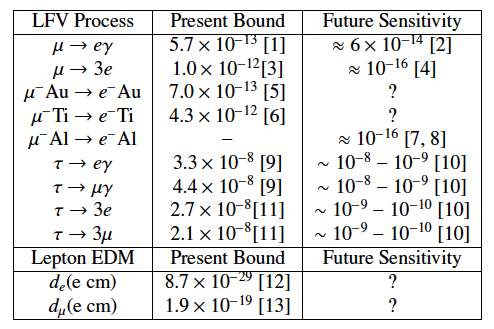
\includegraphics[width=0.6\textwidth]{images/lfv-bounds.png}
\caption{Current experimental limits on various LFV processes}
\label{}
\end{figure}

\section{Hints of LFV beyond the Standard Model}

\subsection{Neutrino mixing}

The discovery that flavour mixing can occur in the neutrino sector proves that neutrinos have mass. Both the concept of massive neutrinos, and by extension the mechanisms which generate neutrino mass, are not predicted or explained by the SM. This tells us that the lepton sector is not fully understood.

There are many NP models which introduce mechanisms to give neutrinos mass. These include SUSY, seesaw models, and many others. In introducing these mechanisms, many of these models inadvertently introduce LFV! As a particle example, a Type-II seesaw model posits a scalar triplet of Higgs-like particles. This triplet comprises a doubly-charged Higgs, a singly-charged Higgs, and a neutral Higgs. As show in Figure X below, lepton-flavour violating processes could proceed via leptons coupling to these scalars!


\begin{figure}[h]
\centering
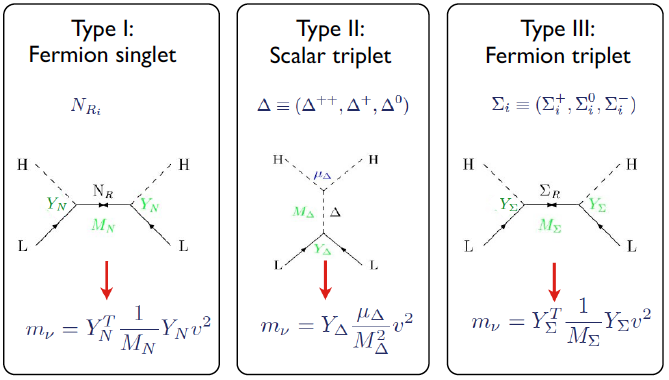
\includegraphics[width=0.5\textwidth]{images/seesaw.png}
\caption{}
\label{}
\end{figure}

\begin{figure}[h]
\centering
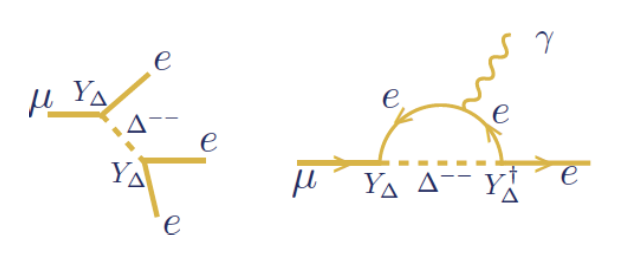
\includegraphics[width=0.5\textwidth]{images/seesaw-lfv-modes.png}
\caption{}
\label{}
\end{figure}




\subsection{$\htm$ excess}

Hints of LFV can come in the form of experimental results which in not consistent with the SM. One such ``anomaly’’ is the $\htm$ excess. In 2015, CMS found a $2.4\sigma$ excess in the branching fraction of $\htm$. This process is lepton flavour violating, so in the SM its branching fraction is predicted to be consistent with zero. However it was determined

\begin{equation}
\br(h\to \tau \mu) = (0.84\pm)\%
\end{equation}


Also in 2015 was a similar search performed by ATLAS, in which an excess of $1.2\sigma$ was found in the $\htm$ decay. 

\begin{equation}
B(\htm) = (0.77 \pm 0.66)\%
\end{equation}

Though this $1.2\sigma$ result is less indicative of NP, it still provides hints as to where NP could occur. These results indicate possible new physics in the Higgs sector! Several models, including Two-Higgs Doublet Models (2HDM), introduce new Higgs-like particles; these particles can couple with leptons to allow lepton flavour violating processes. In fact, LFV can occur naturally in any model with more than one Higgs doublet.


\begin{figure}[h]
\centering
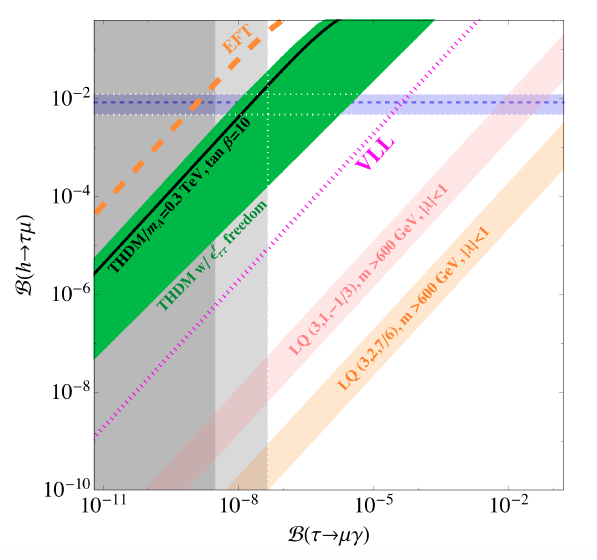
\includegraphics[width=0.5\textwidth]{images/h-vs-tau.png}
\caption{}
\label{}
\end{figure}

\begin{figure}[h]
\centering
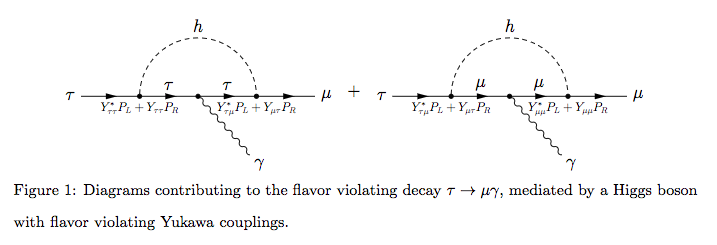
\includegraphics[width=0.5\textwidth]{images/higgs-lfv-modes.png}
\caption{}
\label{}
\end{figure}


\section{Searches for $\tlg$}

The most recent searches for $\tlg$ were undertaken at Belle (2007) and Babar (2010), for both $\ell=\mu,e$ modes.

\subsection{Belle searches}

\subsection{Babar searches}



Other tau LFV modes and their constraints on $\tlg$.


\begin{figure}[h]
\centering
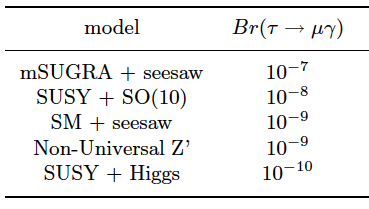
\includegraphics[width=0.5\textwidth]{images/np-models-bounds.png}
\caption{}
\label{}
\end{figure}




\pagebreak

%-----------------------------------------
\bibliographystyle{plain}
\bibliography{refs.bib}
\end{document}







